% 天体运动的简单数值计算
% 天体运动|常微分方程|Matlab|数值计算

\pentry{万有引力\upref{Gravty}, 弹簧振子受迫运动的简单数值计算\upref{SHOFN}}

下面我们来用一种极其简单的算法对单个天体在中心天体的万有引力作用下的运动进行数值计算. 事实上该问题存在解析解(见开普勒三定律\upref{Keple}), 所以以下的算法只是用于演示数值解常微分方程的大致原理. 这种方法可以轻易地拓展到多个天体的情况, 而多体情况没有一般的解析解. 一种效率更高的常见常微分方程数值算法可参考 “四阶龙格库塔法\upref{OdeRK4}”.

直角坐标系中, 设中心天体质量为 $M$, 固定在原点不动.根据牛顿万有引力定律,质量为 $m$ 的行星受到中心天体的力为
\begin{equation}
\bvec F = -G \frac{Mm}{r^2}\uvec r = -G\frac{Mm}{r^3} \bvec r
\end{equation}
其中 $\bvec r$ 为行星的位矢(设行星在 $xy$ 平面上运动). 根据牛顿第二定律\upref{New3}, 加速度为
\begin{equation}
\bvec a = \frac{\bvec F}{m} = -G\frac{M}{r^3} \bvec r
\end{equation}
用 $r = \sqrt{x^2+y^2}$ 以及 $\bvec r = x\uvec x + y\uvec y$, 其中 $x,y$ 看成 $t$ 的函数. 考虑到 $a_x = \ddot x$, $a_y = \ddot y$, 可以列出二阶微分方程组(变量上方两点表示关于时间的二阶导数)
\begin{equation}\label{KPNum0_eq3}
\leftgroup{
\ddot{x} = -\frac{GM}{(x^2+y^2)^{3/2}}x\\
\ddot{y} = -\frac{GM}{(x^2+y^2)^{3/2}}y
}\end{equation}
假设已知初值条件 $x(0) = x_0$, $y(0) = y_0$, $\dot x(0) = v_{x0}$, $\dot y(0) = v_{y0}$. 下面用 “弹簧振子受迫振动的简单数值计算\upref{SHOFN}” 中类似的方法求接下来行星的运动轨迹.

1.将初始条件代入\autoref{KPNum0_eq3},得到初始加速度
\begin{equation}
\leftgroup{
\ddot x(0) &= -\frac{GM}{(x_0^2 + y_0^2)^{3/2}} x_0\\
\ddot y(0) &= -\frac{GM}{(x_0^2 + y_0^2)^{3/2}} y_0
}
\end{equation}
 
2.设经过一段极微小的时间步长 $\Delta t$ (例如 $0.0001$, 数值越小误差越小), 根据微分近似(微分近似在这里的物理意义是在 $\Delta t$ 内速度和加速度都近似为常数)
\begin{equation}
\begin{cases}
\dot x(\Delta t) \approx \ddot x(0)\Delta t + x(0)\\
\dot y(\Delta t) \approx \ddot y(0)\Delta t + \dot y(0)
\end{cases}
\qquad
\begin{cases}
x(\Delta t) \approx \dot x(0)\Delta t + x(0)\\
y(\Delta t) \approx \dot y(0)\Delta t + y(0)
\end{cases}
\end{equation}

3.把 $x(\Delta t), y(\Delta t)$ 再次代入\autoref{KPNum0_eq3}, 得到 $x''(\Delta t), y''(\Delta t)$, 再次利用微分近似求出 $x(2\Delta t), y(2\Delta t), x'(2\Delta t), y'(2\Delta t) \dots$ 如此循环下去就可以得到每隔 $\Delta t$ 的数值解.

\begin{lstlisting}[language=matlab, caption=kepler.m]
% 参数设定
GM = 1; % 万有引力常数乘以中心天体质量
x0 = 1; y0 = 0; % 初始位置
vx0 = 0; vy0 = 0.7; % 初始速度
T = 4; Nstep = 4000; % 总时间和步数
dt = T/Nstep; % 步长

% 矩阵预赋值
x = nan(Nstep,1); y = x;
x1 = x;  y1 = x;
x2 = x; y2 = x;

% 初始位置,速度,加速度
x(1) = x0; y(1) = y0; % 初位置
x1(1) = vx0; y1(1) = vy0; % 初速度
x2(1) = -GM*x(1)/(x(1)^2+y(1)^2)^(3/2); % 代入方程得到 x''(0)
y2(1) = -GM*y(1)/(x(1)^2+y(1)^2)^(3/2); % 代入方程得到 y''(0)

% 迭代循环
for ii = 2:Nstep
    x(ii) = x(ii-1)+x1(ii-1)*dt; % x的微分
    y(ii) = y(ii-1)+y1(ii-1)*dt; % y的微分
    
    x1(ii) = x1(ii-1)+x2(ii-1)*dt; % x' 的微分
    y1(ii) = y1(ii-1)+y2(ii-1)*dt; % y' 的微分

    x2(ii) = -GM*x(ii)/(x(ii)^2+y(ii)^2)^(3/2); % 代入微分方程求出 x''
    y2(ii) = -GM*y(ii)/(x(ii)^2+y(ii)^2)^(3/2); % 代入微分方程求出 y''
end

% 画图
plot(x,y); % 画行星轨道
axis equal; % xy坐标长度一致
hold on; % 继续画图
scatter(0,0); % 标出中心天体
\end{lstlisting}

程序运行结果如\autoref{KPNum0_fig1} 所示. 注意行星轨道并不是一个闭合的椭圆, 这是由于这种算法误差较大, 为了减小误差, 可以增加程序中 \verb|Nstep| 的值.
\begin{figure}[ht]
\centering
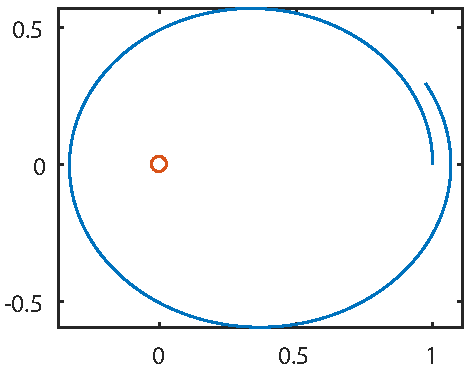
\includegraphics[width=7cm]{./figures/KPNum0_1.pdf}
\caption{运行结果} \label{KPNum0_fig1}
\end{figure}
